\documentclass{article}
\usepackage{graphicx} % Required for inserting images
\usepackage{todonotes}
\usepackage{hyperref}
\usepackage{multicol}
\usepackage{blindtext}
\usepackage{amsmath}
\usepackage{graphicx}
\usepackage{floatpag}
\usepackage{amssymb}
\usepackage{wrapfig}
\usepackage{hyperref}
\usepackage{caption}
\usepackage{algorithm}
\usepackage{algpseudocode}
\usepackage{listings}
\usepackage{color, colortbl}
\usepackage{listings}
\usepackage{emoji}
\usepackage{xcolor}
\usepackage{booktabs}
\usepackage{tabularx}

\definecolor{jsonkey}{RGB}{0,0,128}
\definecolor{jsonstring}{RGB}{0,128,0}
\definecolor{jsonnumber}{RGB}{128,0,0}


\lstdefinelanguage{json}{
  basicstyle=\ttfamily\small,
  stepnumber=1,
  showstringspaces=false,
  breaklines=true,
  backgroundcolor=\color{white},
  commentstyle=\color{gray},
  keywordstyle=\color{jsonkey},
  stringstyle=\color{jsonstring},
  morestring=[b]",
  frame=tb,
  morestring=[d]',
  morecomment=[l]//,
  morecomment=[s]{/*}{*/},
  morekeywords={true,false,null},
  sensitive=true,
}

\lstdefinelanguage{prompt}{
    basicstyle=\ttfamily\small,
    stepnumber=1,
    showstringspaces=false,
    breaklines=true,
    backgroundcolor=\color{white},
    keywordstyle=\color{jsonkey},
    morekeywords={[4]<hl>,<ans>,<ctx>,<question>},
    keywordstyle={[2]\color{purple}\bfseries},
    frame=tb,
}

\lstset{
    breaklines=true
}

\usepackage[backend=biber,style=numeric,sorting=none]{biblatex}
\addbibresource{bibliography.bib}
\title{
    \thispagestyle{empty}
    
\includegraphics[width=0.5\textwidth]{assets/marchio_unipi_pant541.eps}\\[1cm]
    {\Large Human Language Technologies Project Report}\\[1cm]
    {\Large \textbf{Answer-Aware Question Generation: A Comparative Study with Google T5 Transformers and Meta's Llama2}}\\[2cm]
    \large
    \noindent \textbf{Students:} \hfill \textbf{Lecturer:}\\[1ex]
    \noindent Luca Miglior - mat. 580671 \hfill Prof. Giuseppe Attardi\\
    \noindent \raggedright{Vincenzo Gargano - mat. 667591} \\[4cm]
    \midrule
    \noindent
    \date{A.Y. 2022/2023}
}

\date{}
\author{}
\begin{document}
\clearpage
\maketitle
\thispagestyle{empty}
\null\vspace{\fill}
\begin{abstract}
\noindent
This report explores the capabilities of Transformers, especially Sequence To Sequence Large Language models in the task of Answer-Aware question generation. For this project's purposes, we decided to employ Google T5 model for English conditional text generation, in different sizes and with different language modelling approaches. The experimental outcome consistently confirmed the state of the art results obtaining up to 0.92 BERTScore (F1) on T5-Base Transformer (223M parameters) and 41.1 ROUGE-1 with supervised fine tuning. We also assessed Causal Language Modelling performance on Meta's Llama 2, obtaining similar metrics as sequence-to-sequence models, but producing more variegate and accurate questions. Finally we employed Proximal Policy Optimization Reinforcement Learning techniques to lexically and semantically improve models results. The good outcome of this analysis again confirms LLMs helpfulness and power in solving language modelling tasks, that is crucial for practical applications, especially in educative and e-learning settings.
\end{abstract}
\vspace{\fill}

\clearpage
\newpage
\tableofcontents
\newpage
\section{Introduction}
In the era of neural networks and generative models, this report delves into the capabilities of neural models in being able to generate questions for a given topic. The development of an automatic neural question generation system could provide significant advantage and reveal helpful in many fields, especially in education and e-learning settings. The capabilities of generative models of effortlessly analyzing vast amount of text and potentially generating high-quality, semantically appropriated questions for a given topic could play a pivotal role in building tailored and effective education platforms. Moreover, this ability could be seamlessly extended in many other fields, including automated job interview systems with challenging questions and healthcare applications, where diseases can be identified through targeted and highly precise questions about symptoms.

Generally speaking, two main approaches have been adopted in neural question generation problems: End-To-End generative systems \cite{RODRIGUEZTORREALBA2022118258}, where the model is trained to generate questions given a context and a reference question, and Answer-Aware question generation systems \cite{sun-etal-2018-answer}, where the model is trained to produce outputs with the addition of a reference answer related to the reference question.

In this work, our focus will be on the very specific task of Answer-Aware Neural Question Generation. This approach trains models that are more inclined to generate questions related to the provided answers, rather than relying solely on general context-based content. This not only enhances training effectiveness but also improves the overall semantic and syntactic performance of the model. In particular, following the approach proposed in \cite{tang2017question} we will treat the question generation process as a \textit{dual} variation of the question answering process, setting up a training pipeline leveraging the intrinsic probabilistic correlation existing among question and answers for a given context. In particular, this correlation directly comes from the actual joint probability expressed in Equation \ref{eq:jointprob}, where $p(q|a)$ clearly models a probablity distribution of question tokens given an answer $a$. 
\begin{equation}
    p(q, a) = p(q)p(a \vert q) = p(a)p(q \vert a)
    \label{eq:jointprob}
\end{equation}
Practically speaking, what we will propose in this work is approximating the actual probability distribution \( p(q|a) \) with the introduction of a set of trainable parameters \( \theta \), leading to the new distribution \( p(q \vert a, \theta) \approx p(q \vert a) \). This new distribution can be further modeled through the employment of a neural architecture, a choice we will delve into further in the paper.

\section{Related works}
Historically, the neural question generation problem was usually tackled by the employment of Recurrent Neural Networks (RNNs) such as Long-Short Term Memory (LSTM) \cite{lstm} cells or Gated Recurrent Units \cite{gru} based architectures, and has traditionally been modelled as a sequence-to-sequence recurrent problem, in which the recurrent encoder was trained to encode input context sequences in a latent space, and the decoder was trained to generate questions from the summarized inputs enbeddings. This approach poses considerable limitations, given the sequential nature of RNNs and raises further concerns about the reliability of the proposed architecture when processing long-context sequences. In order to be able to process longer sequences, we follow the approach proposed by Chan et al. \cite{chan-fan-2019-recurrent}, by employing attention based transformers models \cite{DBLP:journals/corr/VaswaniSPUJGKP17}, widely recognized as the state of the art architectures for language modelling. The authors have successfully developed a recurrent BERT architecture, effective in predicting masked tokens by taking into account the preceding context. This architecture excels in generating semantically accurate, context-aware questions. Furthermore, the authors introduce the concept of answer-token highlighting within the context, enhancing the model's ability to process longer text sequences and generate questions of significantly improved quality.

\section{Dataset Analysis and Data Preparation}

\begin{figure}[ht]
\begin{lstlisting}[language=json]
{   
    id: "57379829c3c5551400e51f3f"
    title: "Force" 
    context: "The weak force is due to the exchange of the heavy W and Z bosons. Its most familiar effect is beta decay (of neutrons in atomic nuclei) and the associated radioactivity. The word 'weak' derives from the fact that the field strength is some 1013 times less than that of the strong force. Still, it is stronger than gravity over short distances. A consistent electroweak theory has also been developed, which shows that electromagnetic forces and the weak force are indistinguishable at a temperatures in excess of approximately 1015 kelvins. Such temperatures have been probed in modern particle accelerators and show the conditions of the universe in the early moments of the Big Bang."
    question: "What is the effect of beta decay?"
    answer: { 
        text: ["radioactivity"], 
        answer_start: [156] 
    }
}
\end{lstlisting}
\caption{SQuAD dataset physics-related example, reported in json format. The field \texttt{answer\_start} indicates the index of the first occurrence of answer in the context. }
\label{lst:squad}
\end{figure}

In this section, we detail the process of selecting and preparing our dataset in order to assess its integrity and reliability, essential for our investigation into question generation (QG). Our choice fell on the widely recognized Stanford Question Answering Dataset (SQuAD) \cite{rajpurkar-etal-2016-squad}.
The selection of SQuAD as our dataset is mainly related with its reputation, making it an ideal choice for our QG-focused study. The decision was grounded in the dataset's popularity in the research community, ensuring a robust basis for our exploration into question generation methodologies. The SQuAD dataset is composed of over 100K examples, divided across different fields, consisting of questions posed by crowdworkers on a set of 536 English Wikipedia articles, where the answer to every question is a segment of text, or span, from the corresponding reading passage. Nature of the proposed SQuAD question is various. As reported in Figure \ref{lst:squad}, a single dataset sample contains five columns, \texttt{id, title, context, question} and \texttt{answer}; the latter not only containing the single answer to the question, but also indicating the starting index of the answer string in the context. This will be crucial for the future preprocessing steps, as it allowed us to perform finer language modelling and preprocessing steps in a much efficient way. This makes the SQuAD dataset not only precise and reliable, but also usable and effective for our purposes.



\subsection{Preprocessing Pipeline}
In their study, the authors of \cite{chan-fan-2019-recurrent} observed that fine-tuning models with paragraph-level extended contexts led to lower-quality generated questions, even when employing attention-based models. This decrease in quality was attributed to the presence of answer tokens within the same question context, resulting in significant ambiguities and adversely affecting the semantic quality of question generation.

To mitigate this issue, the authors proposed a preprocessing pipeline designed to help BERT models in accurately identifying answers within the context. In order to replicate this pipeline, we applied a fine preprocessing step to the SQuAD dataset. This involved introducing new special tokens for context, questions, answers, and answer highlighting within the text. Formally, given our SQuAD input data, denoted as $X$, we modified it as follows:

\[ X = \textbf{\texttt{ <ctx> }} \text{context} \textbf{\texttt{ <ctx>}} \texttt{<ans> } \text{answer}\]

Here, the new context, represented by $context$, was defined as follows:

\[ \textit{context} = \text{\textit{squad context}}[:as] \textbf{\texttt{ <hl> }} \text{answer text} \textbf{\texttt{ <hl> }} \text{\textit{squad context}[as + l:]} \]

In this context definition, $\textit{squad context}[as:]$ denotes the splitting of the text array into two parts based on the "answer start" information contained in the SQuAD record. The first split is then merged after highlighting, considering the length $l$ of the answer. This preprocessing step aimed to enhance the model's ability to discern answers within the given context, ultimately improving question generation performance from a semantic standpoint.
\begin{figure}
    \centering
    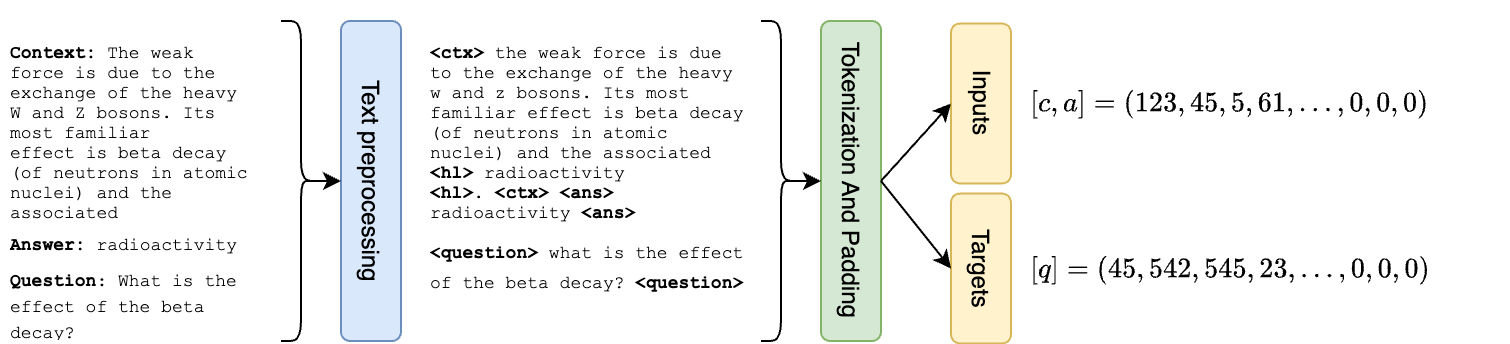
\includegraphics[width=\textwidth]{assets/training-pipeline.drawio.png}
    \caption{Graphical representation of the ``highlight" text preprocessing pipeline}
    \label{fig:preprocessing}
\end{figure}
As final preprocessing steps, we removed upper-case letters and we finally applied tokenization.

To conduct a deep evaluation of our models, we implemented a shuffling and partitioning strategy for the SQuAD dataset, creating distinct subsets for training, validation, and testing. Following a standard split, 80\% of the dataset was allocated for training our models. An additional 10\% of the data served as a validation set to monitor the model's performance and prevent overfitting during training, employing Early Stopping for this purpose. The remaining 10\% constituted our test set, and the evaluation results derived from this set are detailed in Section \ref{experiments}.

\section{Sequence-To-Sequence Language Modelling}
In this section we will describe learning techniques and the applied training pipeline used for training neural generative models. As our first approach, we follow the intuition from \cite{chan-fan-2019-recurrent}, and we decided to set-up a Sequence-to-Sequence (Seq2Seq) Language Modelling training pipeline. 

\subsection{Google T5 and Text-to-Text generation}

In particular, in opposition to the recurrent BERT architecture proposed by the authors, we decided to opt for the more powerful Google T5 encoder-decoder transformer architecture, firstly presented in \cite{t5paper}.In figure \ref{fig:t5diagram} we propose a schematic diagram representing text2text capabilities of T5 model. In our work perspective, T5 model fits perfectly with the goals of our task for several reasons. 
Firstly, the text-to-text design of T5 aligns seamlessly with our objective of generating questions from answers, offering a unified and coherent framework for natural language understanding. Unlike BERT, which relies on masked language modeling, T5's approach treats all NLP tasks uniformly, enhancing its adaptability to diverse language generation tasks. The applied preprocessing pipeline is described in Figure \ref{fig:preprocessing}, where we apply the preprocessing steps onto the example reported in Figure \ref{lst:squad}.

Secondly, the T5 architecture comes pre-trained in a diverse range of tasks and on a larger corpus (C4 dataset, $\approx$750GB corpus \cite{t5paper}). This surely contributes to its ability to capture intricate and more sophisticated linguistic shades. This massive pre-training conveys a deep contextual understanding of language, allowing the model to potentially generate questions that are not only syntactically correct but also semantically rich within the given context.
\begin{figure}[hb]
    \centering
    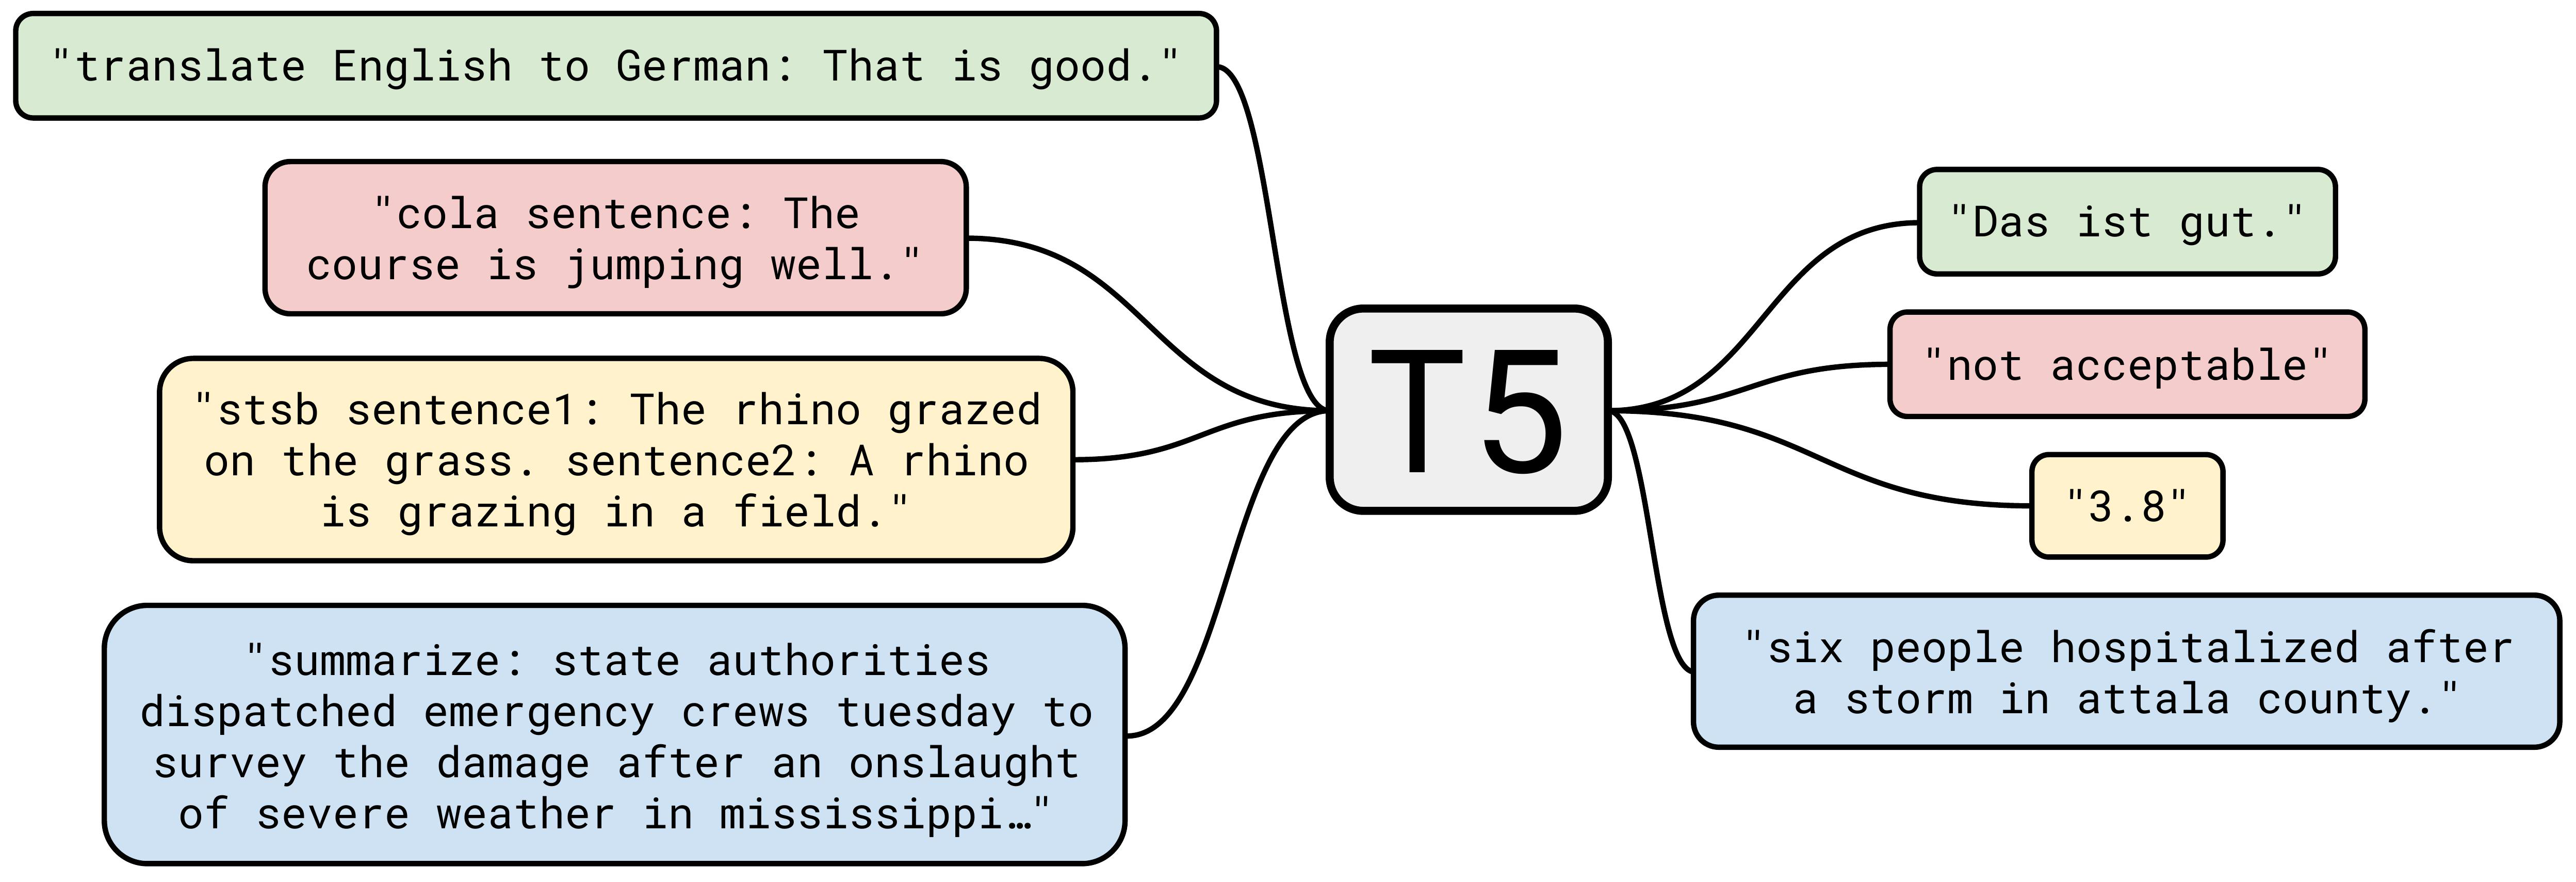
\includegraphics[width=0.8\textwidth]{assets/t5.jpeg}
    \caption{T5 Text2Text diagram from the original paper}
    \label{fig:t5diagram}
\end{figure}
Moreover, T5's transformer architecture presents a larger number of parameters with respect to standard pre-trainerd BERT models, implying higher performance in capturing long-range dependencies in text, a crucial aspect for our task where generating questions requires a comprehensive understanding of the relationship between answers and context. For this study purposes, we decided to test T5 models in small (63M parameters) and base (223M parameters). All T5 models we used were publicly available for usage and downloading on the HuggingFace \emoji{hugging-face} hub.
The assessed success of T5 in various natural language processing benchmarks further affirms its robustness and effectiveness. By leveraging the power of T5, we expect to consistently improve the quality of our answer-aware question generation system, offering a more advanced and contextually rich approach compared to the recurrent BERT architecture. 

\subsection{Weight Quantization and LoRA Efficient Training}

All experiments were conducted on a shared machine equipped with 4x16GB Nvidia P100 GPUs, along with 2x Intel(R) Xeon(R) CPU E5-2698 v4 @ 2.20GHz CPUs (20 cores per socket, 40 logical threads) and 512 GB of RAM. Despite the possibility of accommodating relatively small models like T5-small and T5-base in full precision on the available GPU hardware, we aimed to minimize the training resource footprint. This approach ensures fair utilization of shared resources while expediting both training times and inference.
To achieve this objective, we employed cutting-edge parameter-efficient fine-tuning techniques. For Seq2Seq fine-tuning, our primary optimizations included Weight Quantization, Low-Rank Adaptation (LoRA) \cite{hu2021lora}, and Full Data Parallel for parallelizing training procedures.

\subsubsection{Weights Quantization}

We leveraged the Hugging Face Transformers Parameter Efficient Fine Tuning (PEFT) library to significantly reduce GPU memory usage by quantizing the Language Model's weights during loading. Specifically, all T5 models were loaded with 4-bit precision. This approach allowed us to minimize the model's weight size, ensuring space for training gradients and optimizer states. These states were loaded in half 16-bit precision. Effectively managing gradient memory and optimizer states posed a significant challenge, necessitating the development of complex yet reliable solutions to produce high-quality results within the constraints of limited shared hardware.

\subsubsection{Low-Rank Adaptation}
\begin{figure}[htbp]
    \centering
    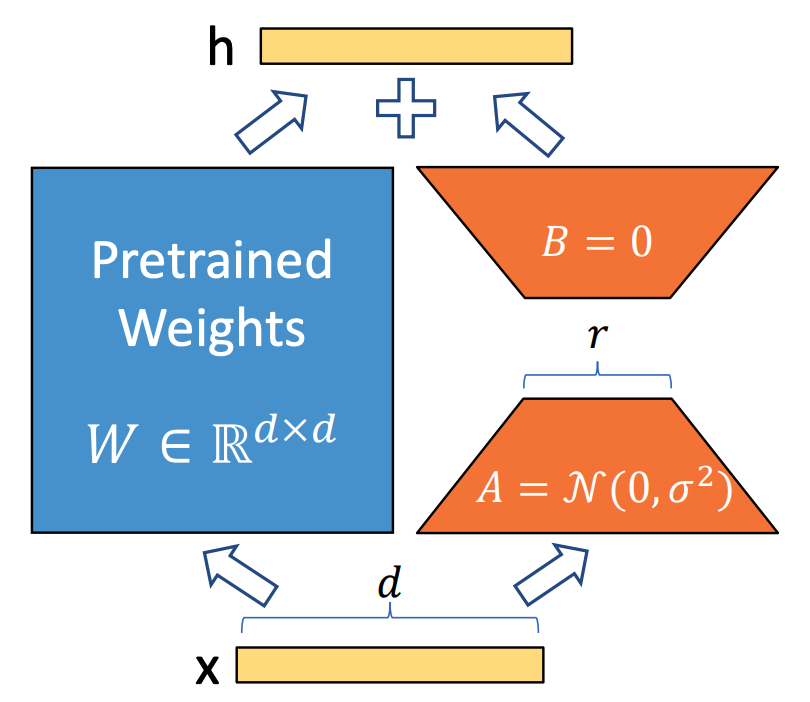
\includegraphics[width=0.5\textwidth]{assets/lora.png}
    \caption{Reparametrization of neural models weight matrix, image from the original paper \cite{hu2021lora}. A and B matrices lay in a low-dimensional subspace, and are initialized with gaussian inizialization and zeroes respectively.}
    \label{fig:lorafig}
\end{figure}

In conjunction with the above mentioned technique, we heavily relied on Low-Rank Adaptation to drastically reduce the number of parameters requiring training, achieving high-quality results with only a fraction of the resources needed for full-rank matrix training.

Neural network outputs, denoted as \(h\), are conventionally computed through vector-matrix multiplications, \(h = Wx\), where \(W\) represents the model's weight matrix, typically full-rank. The study by LoRA authors illustrates how training can be efficiently performed in a much smaller projection of the original matrix subspace, leveraging on the "low intrinsic dimensions" that Language Models show in their weight matrices.

Formally, during LoRA training, the original weight matrix \(W_0 \in \mathbb{R}^{k \times d}\) is decomposed into a smaller representation \(W_0 + \Delta W = W_0 + BA\), where \(B \in \mathbb{R}^{k \times r}\) and \(A \in \mathbb{R}^{r \times d}\), with \(r\) as the user-chosen adaptation rank. Following this approach, the new neural network output \(h\) can be computed as shown in Equation \ref{eq:lora-output}.
\begin{equation}
    h = W_0x + \Delta Wx = W_0x + BAx
    \label{eq:lora-output}
\end{equation}
We propose a graphical representation of how LoRA works in Figure \ref{fig:lorafig}.


This decomposition allows the model weight \(W_0\) to remain frozen during training, with optimization steps performed solely on the scaled and trainable \(\Delta W\) matrix. Throughout our experiments, we successfully trained billion-scale models exclusively on consumer-grade, heavily loaded GPUs, affirming the robustness and innovation of this technique. This achievement not only shows its immediate applicability but also points towards a future where energy consumption is reduced, and access to Large Language Models becomes more accessible to a everyone.


\subsection{Training pipeline}

With the chosen architecture and preprocessing in mind, we proceeded to train the chosen models by leveraging on the help of the PyTorch library and the Huggingface\emoji{hugging-face} Transformers package. All project's codebase was entirely written in the Python programming language. During the training procedure we optimized model weights in order to match datasets' outputs targets. In particular, we chose for a mini-batch training procedure, in order to fully exploit GPU parallelization. As any standard Seq2Seq LM task, our training loop was set up to minimize the cross entropy (CE) loss function among inputs and targets. During the training procedure, we constantly assessed model performance on the validation set every 300 training steps, in order to prevent model overfitting. In particular, we stopped training by the usage of Early Stopping technique, monitoring validation loss as stopping criterion, also setting an improving tolerance of 1\%. As optimizer, we opted for the widely used AdamW \cite{adamw}, with the L2 regularization parameter set to 0.05. We saved optimizer states use floating point half precision gradient computation, in order to save memory during optimization steps. We set the starting value of our learning rate in $1e-4$. Our models were fine-tunied for a duration of 10 complete epochs. Subsequently, the early stopping mechanism was triggered due to the insufficient improvement in the validation loss, indicating a point where further training did not yield significant performance gains.
\begin{table}[h]
\centering
    \begin{tabular}{lccc}
    \toprule
    \midrule
    Model & Epochs & TR Loss (CE) & VL Loss (CE) \\
    \midrule
    T5 base (highlight pipeline)  & 9    & 0.73 & 0.65 \\
    T5 base                       & 9    & 0.76 & 0.71 \\
    T5 small (highlight pipeline) & 10   & 0.81 & 0.86 \\
    T5 small                      & 10   & 0.88 & 0.87 \\
    \bottomrule
        
    \end{tabular}
    
    \caption{Final T5 Losses after models training. It is clear how the text highlighting pipeline produced significant improvements in terms of predictive capabilities. As expected T5-base model nearly outperformed small sized models.}
    \label{table:losses}
\end{table}

\begin{figure}
    \centering
    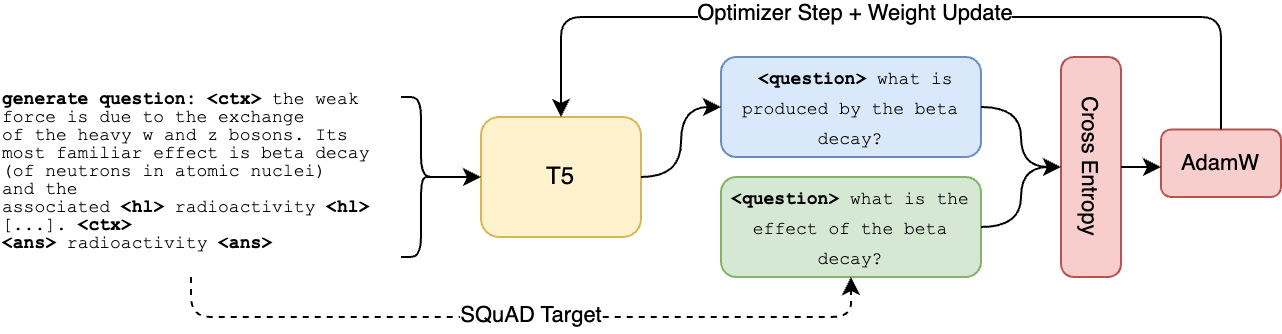
\includegraphics[width=\textwidth]{assets/training-loop.drawio.png}
    \caption{Graphical representation of the training pipeline for a single sample taken from the squad dataset.}
    \label{fig:trpipeline}
\end{figure}
The ``highlighted" training pipeline we adopted could be fairly summarized by Figure \ref{fig:trpipeline}. Starting from the left side, we first preprocess a batch of text and separe the inputs $[ctx, ans]$ from the target $[qst]$. After that, we generate model predictions (center, blue pane) and compute cross entropy loss by comparing the actual SQuAD preprocessed question with our model's output. Finally, we compute weight's gradients and proceed to perform the weight update (right). We replicated this training procedure for each architecture, conducting tests on both datasets, with and without answer highlighting: a total of four models were trained, two T5 small, and two T5-base. Training times for T5 base assessed around five hours on the whole SQuAD datasets, with full data parallel acceleration. Final loss values are reported in Table \ref{table:losses}.

\section{Reinforcement Learning with Proximal Policy optimization}
In this section, we present the application of Reinforcement Learning (RL) and the utilization of Proximal Policy Optimization (PPO) \cite{schulman2017proximal}. Notably, as observed during our experimentation and model evaluations, even the best-performing models exhibited challenges in generating certain questions. Despite the absence of conclusive evidence showing a strong correlation between specific topics and inaccurately generated questions, we try to address these issues using RL. The primary objective behind our choice was to align the distribution of questions in the data with the distribution of questions generated by the model. This strategic approach aims to mitigate instances where generated questions inadvertently contain their answers or when semantically incorrect or contextually inappropriate questions are produced.


\subsection{Mathematical Framework}
Proximal Policy Optimization technique falls into the general category of policy gradient methods (PG) and Actor-Critic (A2C), and is the standard technique employed for PG methods. In particular, in this Language Modelling setting, we can define our policy $\pi_\theta$ as the probability distribution of tokens (the "action"), given a context, i.e. our fine-tuned language models. 
Given a $\theta$ parameterized policy $\pi_\theta(a_t \vert s_t)$, PPO revolves around the idea of gradually aligning the distribution of our model to those of the generated data, alternating sampling from the actual policy and then performing several batch optimization steps through Stochastic Gradient Ascent. This alternation between policy sampling and optimization is equivalent to other methods, but involves lower complexity operations and requires less implementation effort, especially if compared to the well-known Trust Region Policy Optimization (TRPO)\cite{trpo} method that notably presents (empirically) lower data efficiency along second-order optimization and Kullback-Leiber (KL) constraints, often performed by Conjugate Gradient Methods.
With this premises, we move on describing  the General RL policy gradient optimization methods, where the policy objective could generally be defined as follows stated in Equation \ref{eq:policy-gradient-obj}, where the $\log(\pi_{\theta}(a_t|s_t))$ is the log probability of taking an action given the state and the second term $\hat{A_t}$ is a noisy estimate of the \textbf{Advantage Function}.
\begin{equation}
    L^{PG}(\theta) = \hat{\mathbb{E}}_t[\log(\pi_{\theta}(a_t|s_t)\hat{A}_t] 
    \label{eq:policy-gradient-obj}
\end{equation}
In particular, Proximal Policy Optimization defines a probability ratio $r_t(\theta)$ (Equation \ref{eq:ratio}), determining the actual advantage of the current $\pi_{\theta,new}(a \vert s)$ with respect the previous $\pi_{\theta,old}(a \vert s)$.
\begin{equation}
    r_t(\theta) = \frac{\pi_{new}(a|s)}{\pi_{old}(a|s)}
    \label{eq:ratio}
\end{equation}
\noindent
The final \textbf{Clipped} surrogate objective function is finally obtained by the authors as reported in Equation \ref{eq:clipped}, taking the minimum between the normal policy gradient objective and one clipped.
\begin{equation}
    \mathcal{L}^{CLIP}(\theta) = \mathbb{\hat{E}}_t[\min(r_t(\theta)\hat{A_t},clip(r_t(\theta), 1-\epsilon, 1+\epsilon)\hat{A_t})]
    \label{eq:clipped}
\end{equation}
\noindent
The main change introduced by PPO is the direct clipped objective optimization between $[1-\epsilon, 1+\epsilon]$, this has been shown to perform better, because it prevents the actual optimizer to take too large optimization steps if large advantages are met $\hat{A_t}$. In this way,  PPO clips the advantage directly in a proper defined range. 

Practically speaking, our PPO implementation performed the optimization step by solving another alternative formulation of Expectation-Maximization TRPO-inspired problem. In particular, given a reference model (our fine-tuned T5) and the model we want to train, our objective function can be expressed in terms of Equation \ref{eq:ratio} and a Kullback-Leiber penalty term replacing the clipping gradient. Our final PPO objective can be thus expressed as the unconstrained optimization problem driven by Equation \ref{eq:klpenalty}.
\begin{equation}
    \max_{\theta} \text{ }\mathbb{\hat{E}}_t[r_t(\theta)\hat{A_t} - \beta\mathbb{KL}[\pi_{\theta}^{ref}(a\vert s), \pi_{\theta}(a\vert s)]]
    \label{eq:klpenalty}
\end{equation}

\subsection{Reward function Engineering}
\label{reward_function_eng}
Notably, conventional Reinforcement Learning implementations require a suitable reward model to assign appropriate rewards based on the policy distribution. In general, we identified two main approaches for assigning policy rewards in Reinforcement Learning (RL) settings.

The first and simplest approach involves manually engineering a reward function based on the expected policy outcome. Alternatively, the second methodology entails training another model, referred to as a \textit{reward model}, to assess the score for a given action of the objective policy. In the scope of Natural Language Processing (NLP), this approach is commonly employed in LLM training and falls under the category of Reinforcement Learning with Human Feedback (RLHF). This involves training a LLM to act as an human annotator after collecting a sufficiently large dataset containing inputs, targets, and human annotations.

Due to the limitations caused by the absence of sufficient data and the high complexity associated with setting up a RLHF pipeline to train such a model, we opted for the first approach. We manually developed a reward function that reflects our model outputs' desiderata. Our reward function operates on provided examples, incorporating contextual information (query), target questions (target), expected answers (answer), and model predictions (prediction). The usual preprocessing steps described in previous sections are applied to both predictions and targets, ensuring compatibility.
The reward computation leverages the BERTScore \cite{bertscore} metric, utilizing the "RoBERTa" \cite{devlin2019bert} model for comparing predictions and targets in English. The resultant F1 score serves as the baseline reward, reflecting the alignment between the model-generated question and the target question.
In addition to the core reward calculation, we introduced three penalty mechanisms to further guide the model's behavior:
\begin{itemize}
    \item \textbf{Question Word Penalty (QWP)}: Our analysis revealed that the vast majority of questions start with a ``question word" (e.g., what, when, where, who). This penalty term assigns a positive 0.5 score if the predicted output's first word matches the target sentence; otherwise, a negative 0.5 score is assigned.
    \item \textbf{Question Length Penalty (QLP)}: A negative 0.5 is assigned if the question length exceeds 32 words, and a positive 0.5 score is assigned otherwise.
    \item \textbf{Answer-In-Question Penalty (AQ)}: A negative 1 is assigned if answer tokens are found inside the prediction string, and a positive 1 if the question does not contain the answer. This represents a significant mistake, warranting a higher penalty.
\end{itemize} 
This comprehensive approach to reward computation and penalty mechanisms aims to guide the model towards generating more contextually appropriate and semantically accurate questions.

To ensure that the final reward falls within a normalized range between 0 and 1, the computed reward is passed through a sigmoid function. This step facilitates consistent and interpretable reward values for the reinforcement learning process.
The final obtained formulation of the reward function for a given input $answer, reference, prediction$ is described in equation \ref{eq:reward}
\begin{equation}
    \hat{A}(a, r, p) = \sigma(\text{BERTScore}(r, p) + \text{QWP}(r,p) + \text{QLP}(q) + \text{AQ}(a, p)
    \label{eq:reward}
\end{equation}
where $\sigma$ denotes the logistic sigmoid function and QP, QWP and LP denotes penalties introduced for answer-in-question errors, question word mismatch and length.

\subsection{Reinforcment Learning pipeline}

\begin{figure}[h!]
    \centering
    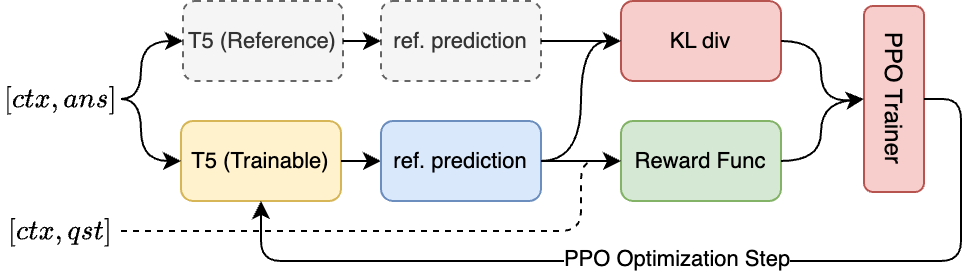
\includegraphics[width=\linewidth]{assets/rl-loop.drawio.png}
    \caption{Modified Training pipeline for Proximal Policy Optimization Reinforcment Learning.}
    \label{fig:ppo-pipeline}
\end{figure}
Within the standard LLM-RL generally entails two crucial steps. In fact, in the standard training pipeline of RL, the first step is Supervised Fine Tuning of a pre-trained architecture. In our specific case, we decided to directly use our T5 fine tuned model. Moreover, we will also use this model as reference policy in order to solve PPO optimization problem.

For the PPO fine tuning step, we set up a training loop focused on maximising the expected value of the reward function. As per the Seq2Seq modelling, we relied on the HuggingFace\emoji{hugging-face} Transformers Reinforcement Learning (TRL) library, providing an effective solution for fine tune transformers with RL. In figure \ref{fig:ppo-pipeline}, we modified the training pipeline for this new paradigm. At each PPO step, each step we take a batch of samples [\textit{ctx,ans}] and compare tokens log-probabilities generated by the trainable model (Bottom row) with the ones reference model one using the KL divergence. This comparison is necessary to compute the KL penalty term in order to prevent the trainable model to take too big optimization steps; next, we decode trainable model's predictions and submit them to the reward function: this will return rewards for the current step (green block). Finally the PPO Trainer takes the computed KL between the models and the rewards generated at time step $t$ and performs the optimization step on the trainable model.



As for the Seq2Seq model, we decided to use AdamW as optimizer, and we set a batch size of 16, learning rate 1e-4, 3 epochs.

\section{Using the big guns: fine tuning a causal billion-sized model}
In this section we will propose an advancement with respect to standard pipeline identified so far. In order to try to overcome the limits and capabilities of million-sized Sequence-to-Sequence transformers, we decided to adopt a totally different approach and proceed with Causal Language Modelling for question generation. We will firstly describe the model choice procedure; after that, we will adapt the Seq2Seq training pipeline to make it adapt to the newer task. Finally we will proceed to evaluate model's result with respect to standard Seq2Seq LM.

\subsection{LLaMA 2 Causal LM}
As the first challenge in the era of Billion-Sized LLMs, we had to face the actual choice of our elective model. After careful analysis, we decided to opt for Meta's new Llama2 \cite{touvron2023llama2}, the direct successor of Llama \cite{touvron2023llama}. Two main reasons led us to this choice. Firstly, this model is publicly available and downloadable from Meta AI's website, in different formats and sizes. Secondly, its performance concerning the number of parameters stands out. In particular, Meta's benchmarks state Llama2's 13B superiority in most benchmarks when compared to OpenAI's 175B GPT-3. Since we had very limited resources for training billion-size models, we decided to opt for 7B version.  

\subsection{Training Billion size models with consumer hardware}
In contrast to our previous experiments with million-sized parameters, where we employed data parallelism to parallelize the batch across GPUs, the transition to billion-sized parameters imposed a strong paradigm shift. Specifically, we moved from the data parallelism to a novel approach: parallelizing the model's weights across GPUs. The challenges associated with training such large models on quasi-consumer, shared hardware became pronounced during the development and conclusion of these experiments. Notably, the constrained memory available in the shared environment posed significant challenges, requiring a modification of our training paradigm to accommodate the scale-up in model size. Moreover, at training time, we also needed a way to reduce size and parallelize optimizer's states and internal variables, as well as gradients. 

In tackling the task of training our model with limited resources, we found DeepSpeed library as a decisive solution. Developed by Microsoft, DeepSpeed emerged as a game-changer in our objective of overcoming memory constraints and parallelizing model weights across GPUs efficiently. By seamlessly integrating DeepSpeed into our workflow, we not only removed memory bottlenecks but also introduced a highly effective approach to distributed and efficient training. 
\begin{figure}[ht]
    \centering
    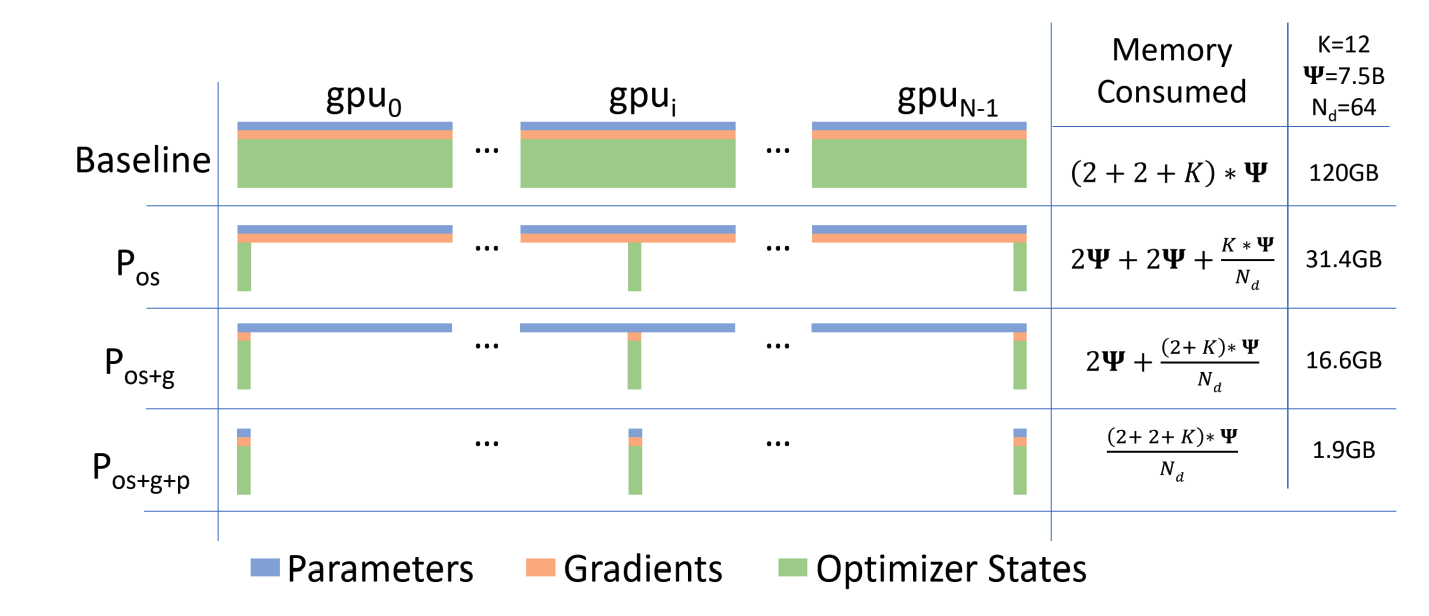
\includegraphics[width=\linewidth]{assets/zero-opt.png}
    \caption{DeepSpeed ZeRO levels of optimizations, image from \cite{rajbhandari2020zero}.}
    \label{fig:zero}
\end{figure}

In addition to the LoRA PEFT configuration and model weights' quantization, we successfully integrated Deepspeed's Zero Redundancy Optimizer (ZeRO) into our training pipeline \cite{rajbhandari2020zero}. This family of optimizers offers three distinct levels of optimization, as illustrated in Figure \ref{fig:zero}:

\begin{itemize}
    \item ZeRO 1 optimization, involving optimizer state (Top row).
    \item ZeRO 2 optimization, incorporating gradient partitioning (Middle row).
    \item ZeRO 3 optimization, encompassing model weight parallelization (Bottom row).
\end{itemize}

To further reduce the memory and resource footprint of ZeRO 3, we opted to enable model parameter CPU offloading and gradient quantization. However, it's important to note that these optimizations come at a cost: while the previous full-data-parallelism employed for T5 fine-tuning resulted in significantly lower training times, the implementation of ZeRO 3 introduces notable overheads in terms of both training and evaluation speeds. We believed that this compromise was a necessary trade-off to harness the benefits of ZeRO 3's advanced optimizations while managing the challenges associated with memory and resources. 

\subsubsection{Instruction tuning}
\begin{figure}[ht]
    \centering
\begin{lstlisting}[label=lst:prompt, language=prompt]
<s>
[INST] 
You are a question generation system. Generate questions for the given answer <answer>, matching the context. Each question starts after <question> and starts with a question word like ``who, what, where, when". [\INST]<ctx> ``The weak force is due to the exchange of the heavy W and Z bosons. Its most familiar effect is beta decay (of neutrons in atomic nuclei) and the associated <hl> radioactivity <hl> . The word 'weak' derives from the fact that the field strength is some 1013 times less than that of the strong force. <ctx> <ans> radioactivity <ans> <question> what is the effect of beta decay? <question> 
<\s>
\end{lstlisting}
    \caption{Instruction prompt used for question generation with Causal Llama model. }
    \label{fig:prompt}
\end{figure}

\noindent
As required by this change in paradigm, in order to train a Causal LM, we decided to slightly modify the previous discussed preprocessing pipeline. In this scenario, instruction tuning emerged as a promising solution for fine-tuning LLMs to perform desired tasks or generate targeted outputs. This approach involves explicitly guiding the LLM's behavior by providing instructions or prompts that clearly define the desired outcome. These instructions serve as a roadmap for the LLM, directing its attention and ensuring that its responses align with the desired objectives.
In particular, we decided to keep the existing preprocessed dataset, but we introduced two special tokens \texttt{[INST]}, \texttt{[\textbackslash INST]} for delimiting and highlight the instruction prompt.
Moreover, we needed to manually add start and EOS tokens, as suggested by Llama prompt tuning guide. A sample of the final prompt for fine Llama fine tuning is described in Figure \ref{fig:prompt}.

\subsection{Training}
In this experiment, we employed a training pipeline analogous to the one proposed for sequence-to-sequence models, with necessary modifications to accommodate the utilization of DeepSpeed Zero3 optimizers. The adaptation primarily involved adjusting the training loop to interface seamlessly with the new optimizer architecture. Model weights were updated utilizing the AdamW optimization algorithm with a learning rate of 1e-5 and a weight decay of 0.05.
Hardware limitations imposed stringent limitations on our batch size, restricting it to 2 due to memory constraints. Despite these challenges, we successfully fine-tuned our model using the complete SQuAD training dataset split. The fine-tuning process was accomplished within approximately 22 hours, demonstrating the efficiency of our approach.
Moreover, hardware limitations precluded the concurrent execution of Proximal Policy Optimization (PPO)\footnote{Actually, this was our first aim. Moreover, we also wanted to test RL pipeline with Direct Preference Optimization} on Llama. This is primarily due from the necessity of a second model to serve as a reference model, a requisite component for PPO implementation.

\section{Experimental Results}
In this section, we will delve into the outcomes experiments, focusing not only on raw scores and metrics but emphasizing on the linguistic aspects. We will analyze the correctness of questions concerning both the provided context and answers, evaluating their semantic and syntactic precision. Additionally, our analysis will extend to the richness of vocabulary employed in the generated questions, aiming to offer a comprehensive evaluation of linguistic aspects. Especially, the latter analysis was conducted manually by reviewing random samples generated by each model.
\subsection{Validation pipeline}
As soon as our models finished training, we performed evaluation on the left-out test set. All validation pipeline was set up thanks to the HuggingFace \emoji{hugging-face} pipeline package of the transformers library. 

Since models were trained with LoRA adapters on them, we firstly merged the low-rank adapters in full float precision. After that, we created a script to load models in full 32bit precision for inference. We performed an evaluation of the whole test set for each model, comparing predicted questions with SQuAD references. Moreover, for human evaluation purposes, we sampled 100 random questions to predict, and compared results across models. We will propose a subset of this comparison further in this section. All models predictions were obtained by sampling with a temperature of $1.0$.

\subsection{Evaluation Metrics}
Before proceeding with human evaluation, we opted to conduct a quantitative comparison using popular NLP metrics. Specifically, we chose two main metrics for our project's purposes: Recall-Oriented Understudy for Gisting Evaluation (ROUGE) \cite{lin-2004-rouge} and BERTScore. While these metrics are generally considered accurate as objective performance indicators for models (with higher values indicating better performance), we recognize that they may not be optimal for analyzing our specific outcomes.

Generating questions for a given context and answer involves various approaches, and a low ROUGE value may be associated with a perfectly composed question. Similarly, we noticed that an exceptionally high BERTScore  (our T5-base pretrained model scored 0.81) may be assigned to a question that is entirely incorrect. Consequently, we acknowledge the limitations of relying solely on these metrics to comprehensively assess the quality of our question generation outcomes.

\subsubsection{ROUGE metrics}
ROUGE (Recall-Oriented Understudy for Gisting Evaluation) is a set of metrics widely employed in the field of natural language processing (NLP) and text summarization to assess the quality of generated text by comparing it to reference or ground truth summaries. Developed with a focus on content recall, ROUGE provides a comprehensive evaluation of the overlap and similarity between the system-generated output and the human-created reference summaries. This suite of metrics is particularly valuable for evaluating the effectiveness of algorithms in capturing essential information and maintaining fidelity to the source content.

\begin{itemize}
    \item \textbf{ROUGE-1 (Unigram Recall):}
        Measures the overlap of unigrams (single words) between the system-generated output and reference summaries.
    \item \textbf{ROUGE-2 (Bigram Recall):}
        Examines the presence of bigrams (pairs of consecutive words) in both the system-generated output and reference summaries.
    \item \textbf{ROUGE-L (Longest Common Subsequence):}
        Focuses on the longest common subsequence (LCS) shared between the system-generated output and reference summaries. ROUGE-L evaluates the overall content overlap in the sentences.
    \item \textbf{ROUGE-S (Skip-Bigram Recall):}
    Introduces the concept of skip-bigrams, allowing for a more flexible assessment of word co-occurrence by considering skipped words between pairs.
\end{itemize}

\subsubsection{BERTScore}
BERTScore is a metric designed to evaluate the quality of generated text by leveraging contextual embeddings from pre-trained BERT models. Unlike traditional metrics that rely solely on exact word matches, BERTScore considers the contextual similarity of words and phrases, offering a more precise assessment of the semantic alignment between system-generated outputs and reference summaries. It has gained popularity in natural language processing (NLP) tasks for its ability to capture deep shades in language and semantic equivalence. For our evaluations we used embeddings provided by pre-trained RoBERTa \cite{roberta} model, considering only the F1 score of the obtained precision and recall metrics.

\subsection{Metrics evaluation}
Finally, in Table \ref{tab:metrics_result}, we report the obtained results for all the fine-tuned and tested models. As expected, LLaMA2, due to its massive size in terms of parameters, succeeded in obtaining a higher BERTScore compared to all other models, confirming the ability of Causal LLMs to adapt seamlessly to a large variety of tasks. The notable BERTScore suggests that LLaMA2 excels in capturing semantic shades and contextual information. Notably, our RL-based fine-tuning steps on the T5-base model demonstrated effectiveness, producing slightly better results than its counterpart without reinforcement learning. This indicates that the reinforcement learning approach contributes positively to the generation quality of T5-base, as reflected in the higher scores.
These results again underline the impact of model architecture, size, and fine-tuning techniques on the quality of question generation. Furthermore, the table serves as a valuable reference for assessing the strengths and weaknesses of each model with respect to the chosen evaluation metrics, offering insights into their respective performances.

\begin{table}[h]
\centering
\resizebox{\textwidth}{!}{%
\begin{tabular}{lccccc}
\toprule
\midrule
Model & BERTScore (F1) & Rouge-1 & Rouge-2 & Rouge-L & Rouge-S \\
\midrule
LLaMA 2             & \textbf{0.929} & \textbf{0.451} & \textbf{0.241} & \textbf{0.422} &  \textbf{0.422} \\
T5 Base  (hl, RL)   & 0.918 & 0.457 & 0.242 & 0.422 &  0.422 \\
T5 Base  (hl)       & 0.912 & 0.455 & 0.230 & 0.415 &  0.416 \\
T5 Small (hl)       & 0.902 & 0.414 & 0.192 & 0.380 &  0.381 \\
T5 Base  (no hl)    & 0.901 & 0.413 & 0.198 & 0.378 &  0.377 \\
T5 Small (no hl)    & 0.859 & 0.317 & 0.134 & 0.292 &  0.292 \\
T5 Base  (no ft)    & 0.810 & 0.088 & 0.029 & 0.079 &  0.089 \\
\bottomrule
\end{tabular}%
}
\caption{Experimental results of tested models on test set}
\label{tab:metrics_result}
\end{table}

\subsection{Sampling and evaluating generated questions}
To comprehensively assess the actual performance of the models, we opted for a manual evaluation of their results by looking the produced questions. In particular, we selected a random sample of 100 fixed questions ids, selected from the test set for each model. Throughout this manual analysis, we were able to discern LLaMA's superiority in generating pertinent questions characterized by clear language, rich syntax, and an extensive vocabulary. Since this analysis was expected to be extensive and highly demanding in terms of resources, we will only compare our top 4 models, presented in Table \ref{tab:metrics_result}

The manual evaluation revealed insights into the impact of model size on performance. Despite achieving high metric scores, the T5-small model frequently produced low-quality, context-unrelated questions, even in straightforward cases. According to our expectations, the application of Proximal Policy Optimization positively influenced the T5-base model, resulting in more precise and linguistically rich questions aligned with the given context. Furthermore, all Seq2Seq models encountered difficulties in accurately formulating questions for complex answers, especially when the correct question to be generated was not evident from the context.
This manual examination provided valuable qualitative insights into the nuanced performance characteristics of each model, shedding light on their strengths and limitations in real-world question generation scenarios. In the last part of this subsection, we present some examples of generated questions by each model.
\newline
\newline
\textbf{Context 1}: \textit{``Warsaw is the capital and largest city of Poland. It stands on the Vistula River in east-central Poland, roughly 260 kilometres (160 mi) from the Baltic Sea and 300 kilometres (190 mi) from the Carpathian Mountains. Its population is estimated at 1.740 million residents within a greater metropolitan area of 2.666 million residents, which makes Warsaw the 9th most-populous capital city in the European Union. The city limits cover 516.9 square kilometres (199.6 sq mi), while the metropolitan area covers 6,100.43 square kilometres (2,355.39 sq mi)."}

\begin{table}[h]
\centering
\resizebox{\textwidth}{!}{%
    \begin{tabular}{l}
    \toprule
    \textbf{Target question}: \textit{How many residents does the greater metropolitan area have?} \\
    \midrule 
    \textbf{Answer}: 2.666 million\\
    \midrule
    T5 small: \textit{How much is Warsaw the 9th most-populous capital city in the European Union?}\\
    T5 base: \textit{What is the metropolitan area of Warsaw?} \\
    T5 ppo: \textit{What is the population of Warsaw?}\\
    Llama2: \textit{What is the population of the greater metropolitan area of Warsaw?}\\
    \midrule
    \bottomrule
    \end{tabular}
        }
     \caption{Question Generation Results for Context 1: Llama and PPO-trained T5 answer and context. T5 small and base fail to generate the correct answer.}
    \label{table:q1}
\end{table}

\textbf{Context 2}: \textit{``On 17 May 1899, Tesla moved to Colorado Springs, where he would have room for his high-voltage, high-frequency experiments; his lab was located near Foote Ave. and Kiowa St. He chose this location because the polyphase alternating current power distribution system had been introduced there and he had associates who were willing to give him all the power he needed without charging for it. Upon his arrival, he told reporters that he was conducting wireless telegraphy experiments, transmitting signals from Pikes Peak to Paris. The 1978 book Colorado Springs Notes, 1899\u20131900 contains descriptions of Tesla's experiments. On 15 June 1899, Tesla performed his first experiments at his Colorado Springs lab; he recorded his initial spark length at five inches long, but very thick and noisy."}
\begin{table}[h]
\centering
\resizebox{\textwidth}{!}{%
    \begin{tabular}{l}
    \toprule
    \textbf{Target question}: \textit{What was the recorded length of the first spark?} \\
    \midrule 
    \textbf{Answer}: five inches\\
    \midrule
    T5 small: \textit{How long did Tesla's initial spark length be?}\\
    T5 base: \textit{What was Tesla's initial spark length?} \\
    T5 ppo: \textit{How long was Tesla's initial spark length?}\\
    Llama2: \textit{What was the length of Tesla's first spark?}\\
    \midrule
    \bottomrule
    \end{tabular}
        }
    \caption{Question Generation Results for Context 2: All models, were able to generate the correct question for the given answer and context. T5 small fails to generate a correct syntax.}
    \label{table:q2}
\end{table}
\newline
\newline
\textbf{Context 3}: \textit{``In April 1191 Richard the Lion-hearted left Messina with a large fleet in order to reach Acre. But a storm dispersed the fleet. After some searching, it was discovered that the boat carrying his sister and his fiancée Berengaria was anchored on the south coast of Cyprus, together with the wrecks of several other ships, including the treasure ship. Survivors of the wrecks had been taken prisoner by the island's despot Isaac Komnenos. On 1 May 1191, Richard's fleet arrived in the port of Limassol on Cyprus. He ordered Isaac to release the prisoners and the treasure. Isaac refused, so Richard landed his troops and took Limassol."}

\begin{table}[h]
\centering
\begin{tabularx}{\linewidth}{X}
\toprule
\textbf{Target question}: \textit{Who ruled Cyprus in 1191?} \\
\midrule 
\textbf{Answer}: Isaac Komnenos\\
\midrule
T5 small: \textit{Who was the island's despot?}\\
T5 base: \textit{Who took survivors of the wrecks prisoner?} \\
T5 ppo: \textit{Who took the surviving sailors prisoner?}\\
Llama2: \textit{Who was the despot of Cyprus?}\\
\midrule
\bottomrule
\end{tabularx}
\caption{Question Generation Results for Context 3: All models correctly predict the question and are able to get the context. Nonetheless, Llama's ability to grasp depth context shades and meaning is evident, while T5 models tend to repeat words near the answer.}
\label{table:q3}
\end{table}

\subsection{Proposing generated questions to human reviewers}
In order to achieve a less biased and more accurate estimate, we implemented a simple, but effective, human evaluation pipeline. We divided a sample of 100 questions among five individuals fluent in English, and asked them to assign scores to the questions.

Each reviewer was informed on the neural nature of the questions. Subsequently, we presented each reviewer with a list of four questions, one from each of the models under evaluation, along with the target answer and related context. Reviewers were then asked to assign a score to each question, using a scale ranging from 1 to 5. A score of 1 indicated a completely incorrect question (e.g., the answer not being identifiable from the question, significant grammar and spelling mistakes), while a score of 5 indicated a perfectly formulated question, rich in syntax and vocabulary.
It's important to say that reviewers were intentionally not informed about the sizes of the models or the specific associations between questions and architectures. Questions were labeled as Q1, Q2, Q3, and Q4 for reference.
Although this is a rudimentary and homemade pipeline, we managed to obtain interesting results. Final evaluations are reported in \ref{table:human_evaluation} 
\begin{table}[h]
\centering
\begin{tabular}{lcccc}
\toprule
\textbf{Model} & Llama2 & T5 PPO & T5 Base & T5 Small \\
\midrule
\textbf{Average Score} & 4.19 & 3.79 & 3.26 & 2.41 \\
\bottomrule
\midrule
\end{tabular}
\caption{Average Scores from Human Evaluation}
\label{table:human_evaluation}
\end{table}
Consistently to our expectations, human reviewers assigned scores that actually reflected model's performance. In particular, Llama and T5 (PPO) were correctly identified as the best models, with respect to the other configurations, even if they obtained similar scores and evaluation metrics. It is clear from our results how T5-small model's capabilities were not sufficient to always accomplish this task, especially with longer and complex contexts. On the other side, Llama2, with its seven billion parameters was able to achieve a nearly full score on this task.



\label{experiments}
\section{Conclusions and Future Works}
In this project report we successfully managed to train several transformer models architecture and we had the possibility to confirm state of the art results in Language Modelling tasks. Our models were trained to produce meaningful results, confirming transformer based architecture linguistic ability in processing long sequences of tokens, and to produce semantically accurate questions if given a context. Notably, in Causal Language Modeling, Llama2-7B emerged as a powerful choice for such tasks, despite its relatively small size compared to contemporary language models. Surprisingly, smaller models like T5-base (approximately 220 million parameters) demonstrated results comparable to those produced by the massive Llama architecture. However, as discussed in the previous section, Llama2 exhibited a superior ability in processing the general context, producing questions that more accurately reflected the actual tokens distributions of the given samples.

It is evident that this work has the potential for further enhancement through the exploration and implementation of modern solutions, particularly utilizing newer architectures. For example, to generate high-quality synthetic data, as proposed in \cite{veselovsky2023generating}, leveraging very LLMs such as ChatGPT or GPT-4 could be considered for data augmentation.

Additionally, the absence of appropriately annotated data posed significant limitations in developing a state of the art Reinforcement Learning pipeline. Specifically, having access to such data could have facilitated the training of a robust reward model, enabling the development of a Reinforcement Learning with Human Feedback training pipeline. Remaining on Reinforcement Learning topic, many other approach could be tested: Direct Preference Optimization (DPO) \cite{rafailov2023direct} represents a new and powerful paradigm to train models based on human feedback, leveraging the intrinsic ability of language models to behave as annotators.

\section{Acknowledgments}
We would like to express sincere gratitude to Prof. Giuseppe Attardi and University of Pisa for providing the essential hardware support that was fundamental in the successful completion of this project. The university's commitment to maintaining an effective learning environment has significantly contributed to the depth of our work. It is worth noting that, thanks to this project and support we have not only improved our understanding of the subject matter, but have also had the opportunity to employ cutting-edge technologies during a particularly dynamic period of scientific discoveries in the field of Artificial Intelligence. This experience has not only enriched our academic journey but has also improved our skills in scientific communication and writing. We also would like to thank our friends who helped us in reviewing and scoring questions, we know it was a boring work!
\newpage

\printbibliography[heading=bibintoc]
\end{document}

